\section{Project description}
\label{chapter1}

This project develops a medication dispenser that supports elderly people in
taking their medication regularly and correctly. At the scheduled intake time,
the system sends a push notification reminding the person of the due dose and
then uses a weight sensor to verify whether the correct amount was taken. The
result is shown directly on the device via an RGB LED. The system is
implemented with an ESP32 as the sensor node and a Raspberry Pi 4B as the
gateway, which communicate with each other via encrypted Bluetooth.

\subsection{Problem description}

Many elderly people have to take several medications at fixed times every day.
A typical example is a 71-year-old man living alone. Simple reminders such as an alarm
clock or a push notification only ensure that the person knows that a dose is
due. However, they do not guarantee that the dose is actually taken correctly.
The notification may be overlooked, the dose may be forgotten despite the
reminder, or the container may have been filled incorrectly.

The core problem is therefore that knowing is not the same as acting
correctly. Incorrect dosing (overdose, underdose or a missed dose) poses a
safety-relevant risk to the person's health. In addition, intake times and
medication data are sensitive health data that must be protected accordingly.

\begin{figure}[h]
	\centering
	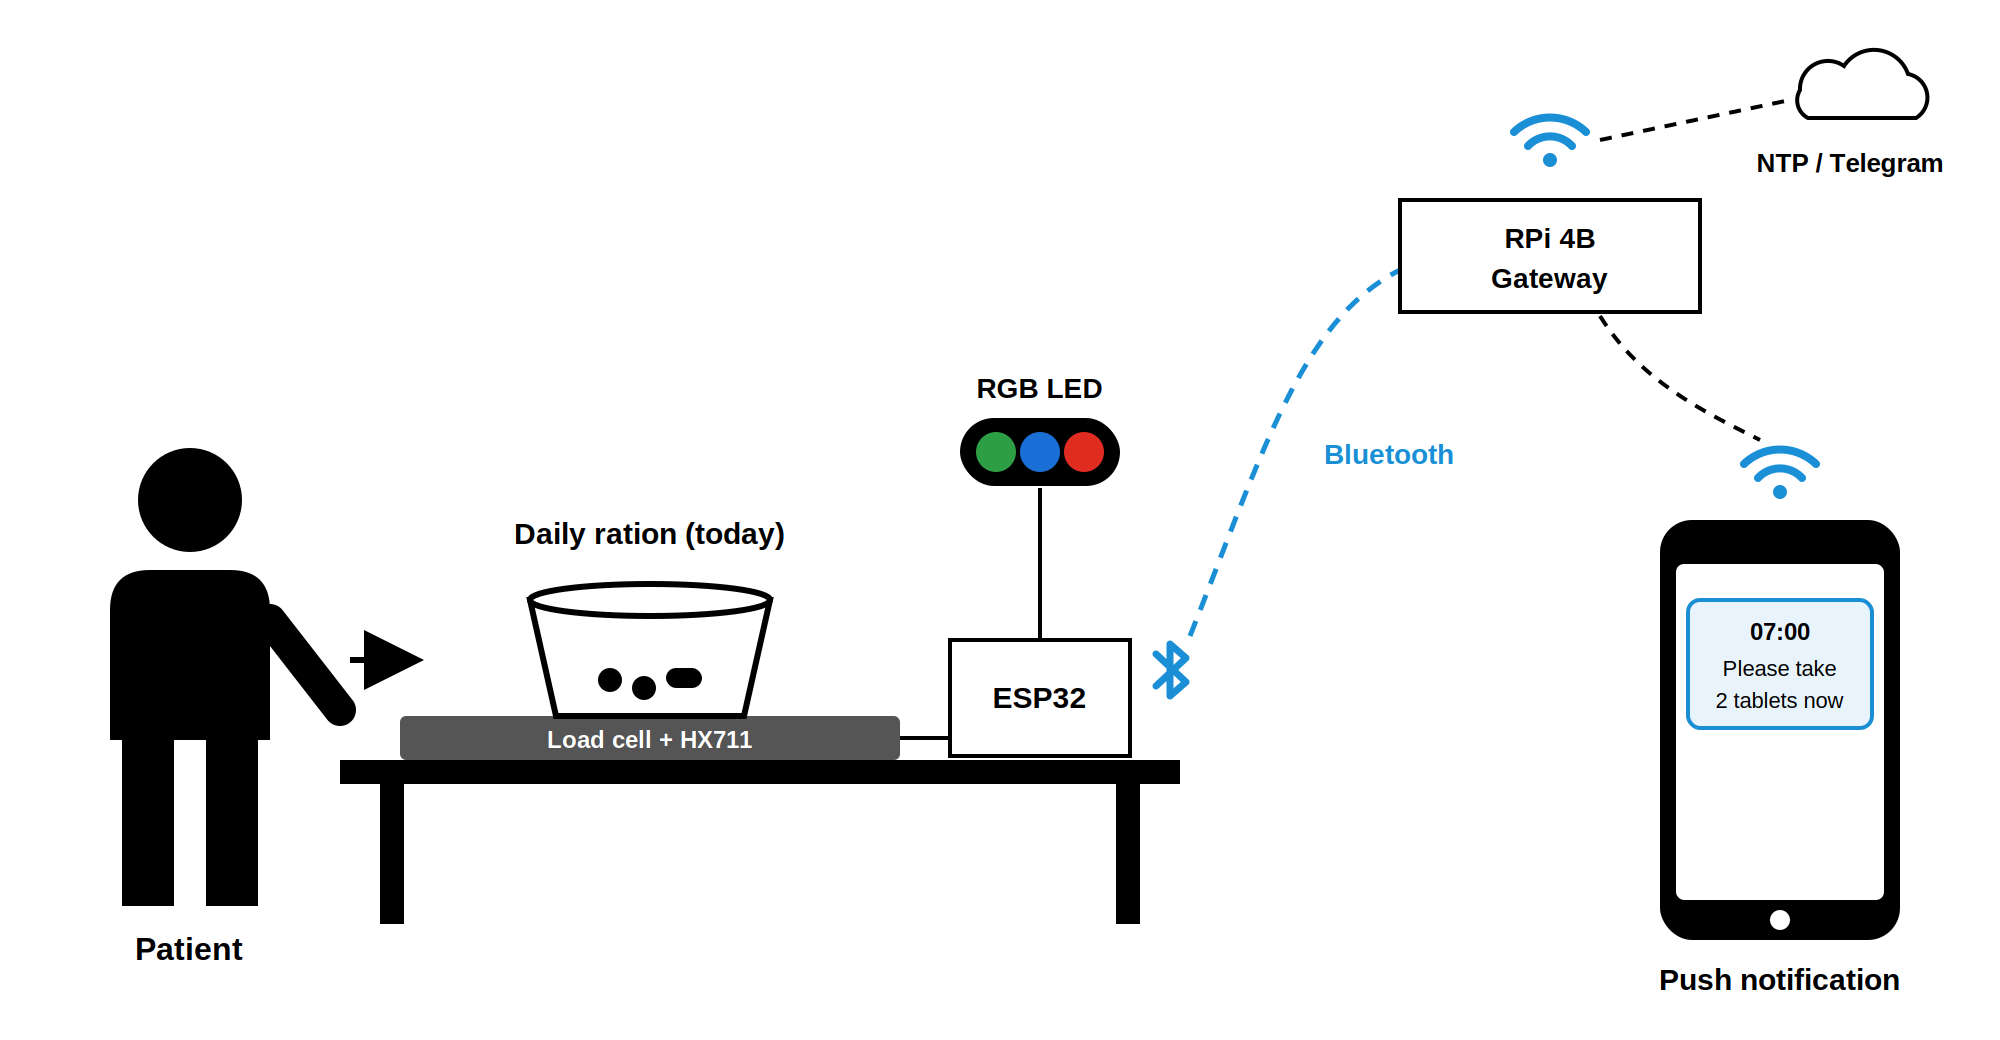
\includegraphics[width=\textwidth]{images/system_overview.png}
	\caption{System description}
	\label{fig:system}
\end{figure}

\subsection{Proposed solution}

The medication dispenser extends the reminder with verified feedback. At the
scheduled intake time, the person receives a push notification on their mobile
phone stating which medications and how many tablets of each have to be
taken (target state). The medication for the current day is
kept in a single container on a weight sensor. Since this container holds the
tablets for all intake times of the day, the notification tells the person
which tablets to take from it at the current intake time.
The weight sensor measures the change in weight when the medication is taken
and thus verifies the action that was actually performed (actual state).

The system operates in a daily cycle. Every morning, the nursing staff fills
the container with the medication for the current day and starts the dispenser
by pressing the reset button (EN) of the ESP32. At start-up, the system checks whether
the container holds the correct amount of medication, i.e.\ whether the
measured weight corresponds to the sum of the target weights of all intake
times of the day. Each intake window starts at the intake time and lasts 1\,h.
At the end of the last intake window of the day, the ESP32 checks whether the
last dose has been taken, reports the end of the day to the Raspberry Pi and
enters deep sleep mode. In this mode, no measurements are performed and the
Bluetooth connection is closed. If the last dose has not been taken, the red LED
remains on during deep sleep, otherwise the LED is off. The ESP32 only wakes up
when the reset button is pressed on the next morning, which starts a new day.
The Raspberry Pi keeps running and waits for the next connection.

The system compares the actual state with the target state and displays the
result via an RGB LED. In addition, the LED indicates faults of the system.
Table~\ref{tab:led} lists all states of the LED.

\begin{table}[H]
	\centering
	\begin{tabular}{|l|p{0.62\textwidth}|}
		\hline
		\textbf{LED} & \textbf{Meaning} \\
		\hline\hline
		Green & The remaining weight corresponds to the expected weight (correct dose taken, also after a missed dose has been taken later). \\
		\hline
		Blue & Deviation from the target weight outside the tolerance, but smaller than the weight of one tablet (e.g.\ measurement inaccuracy). The result is uncertain. \\
		\hline
		Red & Critical state (overdose, underdose, missed dose or medication removed outside an intake window). \\
		\hline
		Red, flashing & Fault due to an incorrect filling at start-up, a sensor fault (see Hazard 2) or a missing valid schedule or time (see Hazard 3). No dose evaluation is performed. \\
		\hline
		Red, green, blue in sequence & LED self-test at program start. \\
		\hline
		Off & Within an intake window until the dose is taken and after the last intake window of the day (all doses taken, no fault present). \\
		\hline
	\end{tabular}
	\caption{States of the RGB LED}
	\label{tab:led}
\end{table}

\subsection{System overview}

The system consists of two microcontrollers (see
Figure~\ref{fig:system}). The ESP32 serves as the sensor node. It reads the
load cell via the HX711 amplifier, detects changes in weight, evaluates the
dose taken and controls the RGB LED (KY-009). Communication with the Raspberry
Pi takes place via Bluetooth. The Raspberry Pi 4B acts as the gateway. It
receives the measurement results from the ESP32, synchronises the time via an
NTP server and sends push notifications via the Telegram Bot API. The intake
schedule is stored in a configuration file on the Raspberry Pi, which is
maintained by the nursing staff. For each intake time, it contains the
medications and their quantity. From this and the weight of one tablet of each
medication, the Raspberry Pi calculates the resulting target weight.